\documentclass[12pt]{article}
\usepackage{hyperref}
%\usepackage[polish]{babel}% <- Dla wersji polskiej



\usepackage[utf8]{inputenc}
\usepackage[T1]{fontenc}
\usepackage{amsmath}
\usepackage{upquote}
\usepackage[margin=2.5cm, bottom=5cm]{geometry}
\usepackage{setspace}
\usepackage{graphicx}
\usepackage{fancyhdr}
\usepackage{pdfpages}
\usepackage{array}
\usepackage{multirow}
\usepackage{float}
\usepackage{comment}
\usepackage{blindtext}
\usepackage{tcolorbox}
\usepackage{soul}

%\pagestyle{fancy}

\usepackage{listings}
\usepackage{xcolor}
\usepackage{changepage}
\usepackage[framemethod=tikz]{mdframed}

% Define colors
\definecolor{codeblue}{RGB}{255, 255, 255}      % Light blue background
\definecolor{keywordcolor}{RGB}{0, 0, 255}      % Blue for keywords
\definecolor{commentcolor}{RGB}{0, 128, 0}      % Green for comments
\definecolor{stringcolor}{RGB}{163, 21, 21}     % Red for strings
\definecolor{numbercolor}{RGB}{0, 0, 0}     % Purple for numbers
\definecolor{numbercolor}{RGB}{0, 0, 0}     % Purple for numbers

% Configure listing style
\lstdefinestyle{mystyle}{
    backgroundcolor=\color{codeblue},
    commentstyle=\color{commentcolor},
    keywordstyle=\color{keywordcolor}\bfseries,
    numberstyle=\color{numbercolor},
    stringstyle=\color{stringcolor},
    basicstyle=\ttfamily\footnotesize,
    breakatwhitespace=false,
    breaklines=false,
    captionpos=t,
    keepspaces=true,
    numbers=left,
    numbersep=5pt,
    showspaces=false,
    showstringspaces=false,
    showtabs=false,
    tabsize=2,
    frame=single,
    rulecolor=\color{codeblue},
    xleftmargin=1.5cm,        % Left margin (2 tabs worth)
    xrightmargin=1cm,       % Right margin for centering
}

% Set the style as default
\lstset{style=mystyle}

% Custom environment for centered code blocks
\newenvironment{centeredcode}
{
    \begin{adjustwidth}{2cm}{2cm}  % Additional centering
    \begin{lstlisting}[language=C]
}
{
    \end{lstlisting}
    \end{adjustwidth}
}

%\title{Discussions on E2E architecture and modeling simplification}
%\date{today}

\begin{document}

%\maketitle

\setlength{\headsep}{3cm}

\begin{center}
%    {\LARGE \textbf{Discussions on E2E architecture and modeling simplification}}\\
%    {\LARGE \textbf{Modernizing E2E Architectures for Earth Observation Missions}}\\
    {\LARGE \textbf{Information-Theoretic Instrument Baseline Design for ISRU Lunar Mineral Mapping}}\\
    {\textbf{\today}}
\end{center}
\begin{center}
    {\textbf{Manfred Gawlas, Jakub Leś}}
\end{center}



\vspace{1cm}

\begin{comment}
\subsection*{Document Approval}
\begin{tabular*}{\textwidth}{|p{3cm}|@{\extracolsep{\fill}}p{4cm}|p{3cm}|p{2cm}|}
\hline
\textbf{Role} & \textbf{Name} & \textbf{Signature} & \textbf{Date} \\
\hline
Author & Manfred Gawlas &  & \today \\
\hline
Reviewer & & & \\
\hline
Approver & & & \\
\hline
\end{tabular*}

\vspace{0.5cm}

\subsection*{Change Record}
\begin{tabular*}{\textwidth}{|p{1.5cm}|p{2.5cm}|p{3cm}|@{\extracolsep{\fill}}p{5.5cm}|p{1.5cm}|}
\hline
\textbf{Version} & \textbf{Date} & \textbf{Author} & \textbf{Description} & \textbf{Sections} \\
\hline
Draft & 22.12.2025 & Manfred Gawlas & Structure and initial text. & All \\
\hline
Draft & 15.01.2026 & Manfred Gawlas & Full thing & All \\
\hline
\end{tabular*}

\end{comment}

\begin{abstract}
With a growing number of lunar prospecting missions entering active development—from ESA-backed initiatives to national programmes such as Poland's Twardowski mission—the debate over optimal payload specifications for In-Situ Resource Utilization (ISRU)-oriented mineral mapping has become increasingly pressing.\\

This study defines detection baselines and minimum instrument specifications required to map all priority ISRU minerals from a single satellite in near-polar lunar orbit, spanning the full 0.4–40 µm spectral range. The target mineral set—drawn from laboratory spectral libraries and including ilmenite, pyrite, troilite, pyrrhotite, fayalite, orthopyroxene, pigeonite, anorthite, hematite, magnetite, akaganeite, apatite, alunite, jarosite, gypsum, anhydrite, and quartz—covers the full range of ISRU-relevant resources: oxide and sulfide minerals as sources of structural metals and chalcophile elements, silicates and feldspars as the dominant regolith background, sulfates as indicators of volatile history, and surface ice and hydrothermal minerals as potential water and propellant sources. Rather than treating this as a single fixed problem, the analysis is conducted across multiple mineral groupings and weighting schemes—for example, grouping basaltic assemblages to reduce spectral unmixing complexity, or prioritising subsets of target minerals according to mission-specific ISRU objectives. Each configuration yields a distinct instrumentation baseline.\\

To determine optimal, minimal spectral band sets for each configuration, we employ an innovative approach combining physically realistic sensor modelling with information-theoretic optimisation. Sensor physics are modelled through wavelength-dependent spectral response functions (dynamic FWHM) and noise variance profiles across the full spectral range, applied to interpolated endmember spectra from the full mineral library. Band selection is then performed via a D-Optimal greedy algorithm that sequentially maximises the marginal gain in Fisher Information, ensuring maximum spectral separability between target and interfering minerals under realistic instrument constraints. This submodular greedy framework provides provable near-optimality guarantees and is applied systematically across all mineral groupings and weighting configurations, generating a family of rigorously scored instrumentation baselines rather than a single solution. The framework additionally incorporates spectral unmixing with per-pixel uncertainty estimation, allowing evaluation of how confidently each baseline can resolve mixed mineral assemblages in realistic regolith scenarios. Alternative optimisation strategies, including Integer Linear Programming and metaheuristic approaches, are under consideration for future comparative evaluation.\\

\begin{figure}[H]
    \centering
    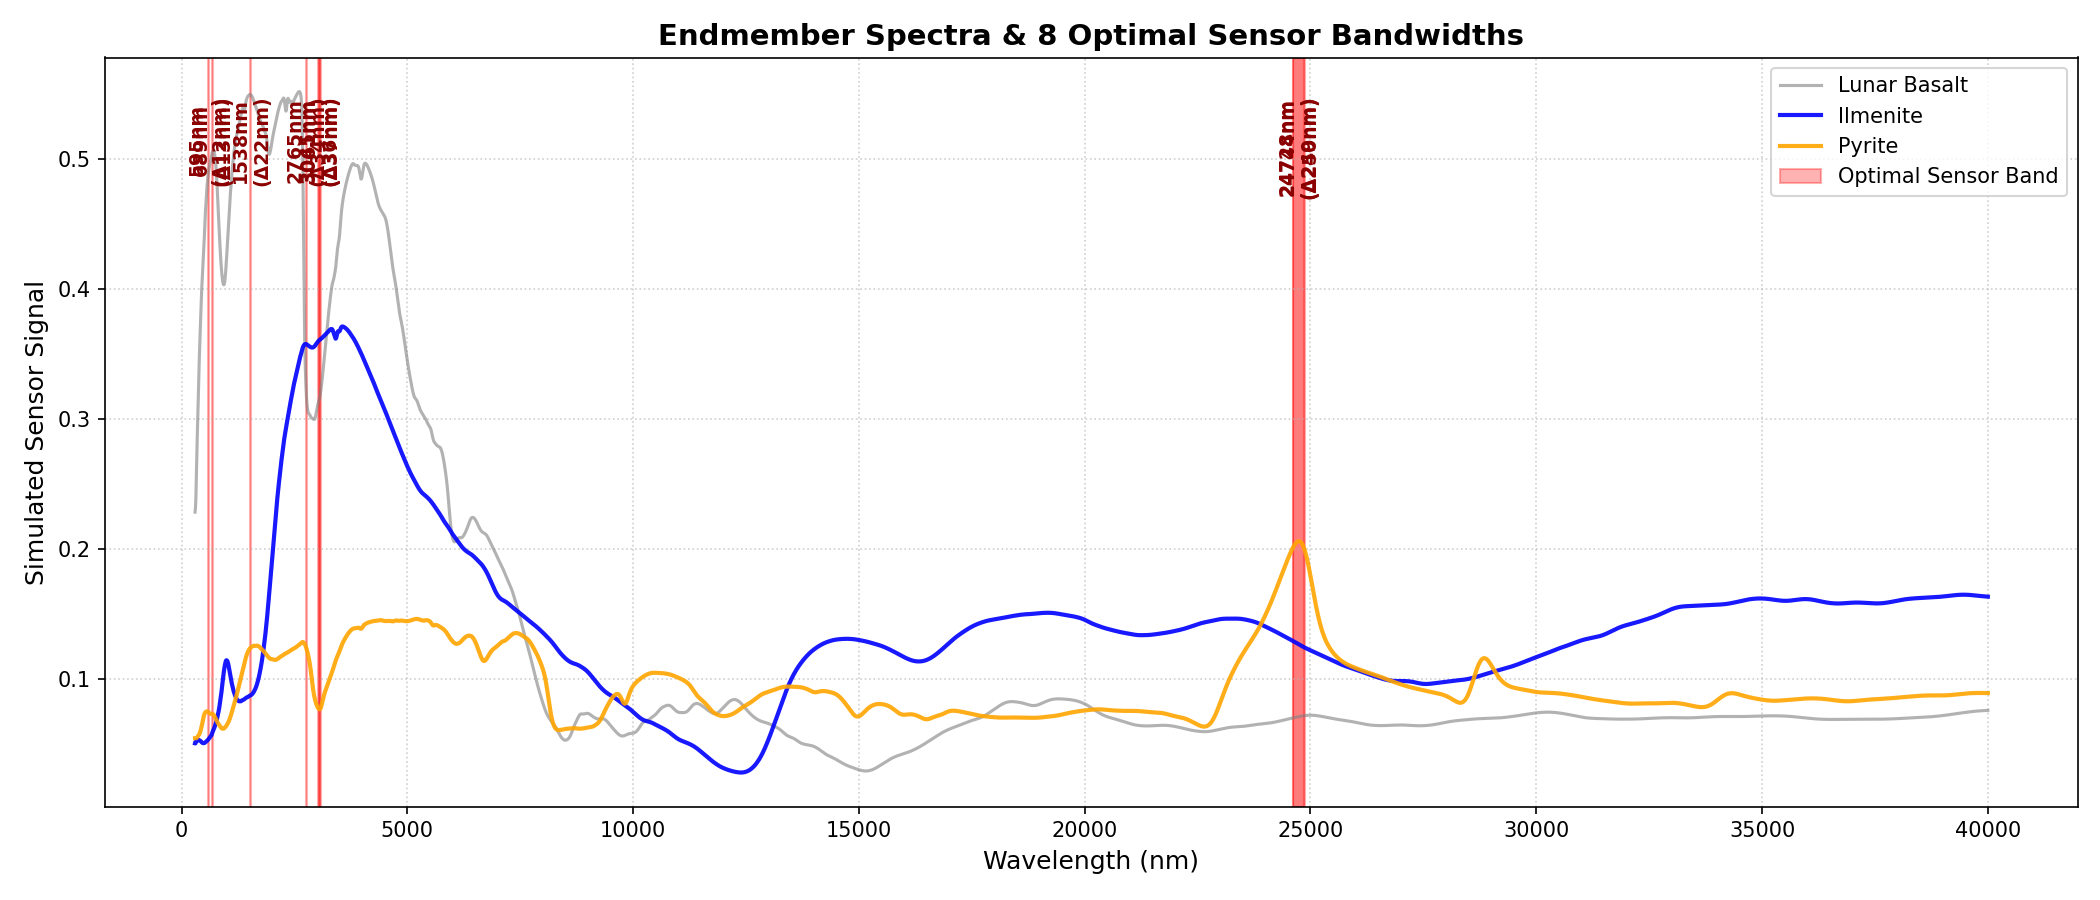
\includegraphics[width=1\textwidth]{img/provable_optimal_bands_FIR.png}
    \caption{Optimal band placement for mineral group of Ilmenite, Pyrite and example lunar basalt.}
    \label{fig:result}
\end{figure}

An example result is shown in Fig. 1, illustrating optimal band placement for one selected mineral grouping, together with the Fisher Information gain landscape and modelled sensor constraints that drove the selection. Results across configurations demonstrate that compact multi-band instruments spanning the VNIR, mid-IR, and FIR can achieve confident discrimination of priority ISRU minerals, with band placement and count varying meaningfully across groupings and noise assumptions.\\

Conclusion to be completed.\\

As lunar resource prospecting transitions from scientific exploration toward mission-critical infrastructure planning, rigorous and reproducible payload specifications become essential. By generating a structured family of quantitative baselines across diverse mission scenarios, this study provides directly applicable guidance for payload designers of the growing number of upcoming lunar mapping missions, and a reusable proven algorithms for future ISRU-oriented instrument definitions.\\
\end{abstract}

%\bibliographystyle{unsrt}
%\bibliography{bib}

\end{document}
